\documentclass[12pt]{article}

\usepackage{amssymb,amsmath}
\usepackage[margin=1.0in]{geometry}
\usepackage{fancyhdr} % required for custom header
\usepackage{graphicx}
\usepackage{listings}
\usepackage{courier}
\usepackage{natbib}
\usepackage{algorithm}
\usepackage{algorithmic}
\usepackage[usenames,dvipsnames]{color}

%set up the header
\pagestyle{fancy}
\lhead{Trever Hines}
\chead{Modeling Seismic Waves}
\rhead{\today}

\setlength{\headheight}{15pt}
\renewcommand\headrulewidth{1.0pt} % Size of the header rule

%% Code inclusion
%%-------------------------------------------------------------------------------
% create a function that import a python script
\lstloadlanguages{Python}
%        frame=single,

\definecolor{blay}{rgb}{0.93,0.93,1.0}
\lstset{language=Python,
        backgroundcolor=\color{blay}, 
        basicstyle=\footnotesize,
        keywordstyle=[1]\color{Blue}\bf,
        commentstyle=\color{Red},
        stringstyle=\color{ForestGreen},
        showstringspaces=false,
        numbers=left,
        numberstyle=\tiny,
        numbersep=3pt,
        stepnumber=2}


\newcommand{\pythonscript}[2]{\begin{itemize}
                              \item[]\lstinputlisting[caption=#2,label=#1]{#1.py}
                              \end{itemize}}

%% Title
%%------------------------------------------------------------------------------
\title{	
AOSS 555 Final Project:\\
Modeling Seismic Wave Propagation with Radial Basis Functions\\
\author{Trever Hines}
\rule{\headwidth}{1.0pt}
}


\begin{document}
\maketitle
\section*{Introduction}
 
In recent years seismologists have become interested in using
observable seismic waveforms to image the elastic properties of the
Earth's interior.  I use the term 'seismic waveform' to refer the the
displacement history that can be observed on a seismogram over the
course of hundreds of seconds following an earthquake.  As with any
inverse problem, imaging the elastic properties of the earth using
seismic waveforms requires one to be able to solve the forward
problem, that is, to compute the waveforms that would be predicted for
a given realization of the Earth's interior.  Researchers have used
various numerical methods to solve this forward problem including
finite difference methods, finite element methods, and spectral
element methods (see \citet{F2011} for a review of numerical methods
in seismology).  In this paper I will explore the potential for using
radial basis functions (RBFs) to solve for the time dependent
displacements throughout the earth following an earthquake.
 
One reason why RBFs are appealing is because they offer freedom in
choosing the collocation points.  In global seismology, one would
ideally have a high clustering of collocation points at the
core-mantle boundary, which is an interfaces where the elastic
properties suddenly and drastically change.  Additionally, the crust
and the core have relatively low velocities and would require a higher
density of nodes in accordance with the CFL criteria.  RBFs seem to be
appropriate for handling such heterogeneity in the Earth.

Another great advantage to RBFs is that they can be used to solve a
problem on an arbitrarily complicated domain.  Although the domain in
global seismology is typically taken to be a sphere or a disk, more
complicated geometries can arise in regional scale seismology problems
where topography may need to be considered.

\section*{Problem Formulation}
We can apply Newton's second law of motion to an infinitesimal parcel
within a continuum to obtain displacements, $\boldsymbol{u}$,
at any point $\boldsymbol{x}$ in the continuum as
\begin{equation}\label{MomentumEquation}
  \rho\frac{\partial^2 u_i}{\partial t^2}  = \frac{\partial \tau_{ij}}{\partial x_j} + f_i,
\end{equation}
where $\boldsymbol{\tau}$ and $\boldsymbol{f}$ are the stress tensor
and body force per unit volume acting on point $\boldsymbol{x}$,
respectively, and $\rho$ is the density at point
$\boldsymbol{x}$. Note that I have adopted Einstein notation where
summations are implied by repeated indices.  We can express
eq. (\ref{MomentumEquation}) in terms of $\boldsymbol{u}$ by using the
definition of infinitesimal strain,
\begin{equation}\label{Strain}
  \varepsilon_{ij} = \frac{1}{2}\left(\frac{\partial u_j}{\partial x_i} + 
                                \frac{\partial u_i}{\partial x_j}\right),
\end{equation}
and Hook's law in an isotropic medium,
\begin{equation}\label{HooksLaw}
  \tau_{ij} = \lambda\delta_{ij}\varepsilon_{kk} + 2\mu\varepsilon_{ij},
\end{equation}
where $\lambda$ and $\mu$ are Lam\'e parameters which we generally
assume to be heterogeneous in the Earth.  The differential equation
being solved is then
\begin{align}\label{DiffEq}
  \rho\frac{\partial^2 u_i}{\partial t^2} &= 
    \frac{\partial}{\partial x_j}\left(\lambda\delta_{ij}\frac{\partial u_k}{\partial x_k} +
    \mu\left(\frac{\partial u_j}{\partial x_i} + \frac{\partial
    u_i}{\partial x_j}\right)\right) + f_i\\\nonumber
  &= 
    \frac{\partial}{\partial x_i}\left(\lambda\frac{\partial u_k}{\partial x_k}\right) +
    \frac{\partial}{\partial x_j}\left(\mu\left(\frac{\partial u_j}{\partial x_i} + \frac{\partial
    u_i}{\partial x_j}\right)\right) + f_i\\\nonumber
  &= 
    \frac{\partial \lambda}{\partial x_i}
    \frac{\partial u_k}{\partial x_k} +
    \lambda\frac{\partial^2 u_k}{\partial x_i x_k} +
    \frac{\partial \mu}{\partial x_j}\frac{\partial u_j}{\partial x_i} +
    \frac{\partial \mu}{\partial x_j}\frac{\partial u_i}{\partial x_j} +
    \mu\frac{\partial^2 u_j}{\partial x_j \partial x_i} + 
    \mu\frac{\partial^2 u_i}{\partial x_j \partial x_j} + f_i.
\end{align}
We impose free-surface boundary conditions, which means that
\begin{equation}\label{BoundaryCondition}
  \boldsymbol{\tau}\cdot\boldsymbol{\hat{n}} = 0
\end{equation}
for all $\boldsymbol{x}$ on the surface of the Earth, which have
surface normal vectors $\boldsymbol{\hat{n}}$.  We can write the
boundary conditions on $\boldsymbol{u}$ more explicitly as
\begin{equation}\label{BoundaryConditionExplicit}
  \hat{n}_i\lambda\frac{\partial u_k}{\partial x_k} +
  \hat{n}_j\mu\left(\frac{\partial u_j}{\partial x_i} +
  \frac{\partial u_i}{\partial x_j}\right) = 0.
\end{equation}

Although the equation that we are trying to solve looks daunting, if
we consider a homogeneous medium, neglect body forces, and assume
that displacement are in one direction and propagate in one direction,
then we can see that eq. (\ref{DiffEq}) reduces to the one dimensional
wave equation. In particular, if displacements are in the direction of
wave propagation then eq. (\ref{DiffEq}) becomes
\begin{equation}\label{1DS}
  \frac{\partial^2 u}{\partial t^2} = \frac{\lambda + 2\mu}{\rho}\frac{\partial^2 u}{\partial x^2},
\end{equation}
where waves propagate at the P wave velocity, $\sqrt{(\lambda +
  2\mu)/\rho}$. If displacements are perpendicular to the direction of
wave propagation then eq. (\ref{DiffEq}) reduces to
\begin{equation}\label{1DP}
  \frac{\partial^2 u}{\partial t^2} = \frac{\mu}{\rho}\frac{\partial^2 u}{\partial x^2},
\end{equation}
where waves propagate at the S wave velocity, $\sqrt{\mu/\rho}$.  

When solving eq. (\ref{DiffEq}), we assume the Earth is initially
stationary and that all displacements are caused by an earthquake.
Earthquakes are a sudden dislocation in the displacement field along a
fault plane and so it seems reasonable that earthquakes should be
imposed in this model by setting appropriate displacement boundary
conditions on a prescribed fault plane.  However, imposing a
dislocation in the displacement field would undoubtedly cause
numerical troubles.  Fortunately, we can instead represent an
earthquake as a collection of slightly offset point force couples,
$\boldsymbol{F}^{(i,j)}$ \citep{AR2002}.  All nine unit force
couples needed to represent a dislocation in three dimensional space
are shown in figure 1. Approximating a dislocation as point force
couples is reasonable if one is concerned with displacements far away
from the source, i.e. seismic waves on a global scale.  The finite
length of a fault rupture must be considered if one is interested in
near field displacements resulting from an earthquake.  Even so,
seismologists routinely represent earthquakes in terms of point force
couples using what is known as a moment tensor, $\boldsymbol{M}$.  The
components of the moment tensor are
\begin{equation}\label{MomentTensorComponents}
  M_{ij} = |\boldsymbol{F}^{(i,j)}|d,
\end{equation}
where $d$ is the offset between the force couples, which would ideally
be infinitesimally small.  To give the moment tensor more tangible
meaning, we can consider an isotropic compression source, such as a
subsurface explosion, where the moment tensor representing that source
would be
\begin{equation}
  \boldsymbol{M} = M_o\boldsymbol{I},
\end{equation}
and $M_o$ is the energy of the explosion. For our numerical
simulation, we imposed an earthquake with moment tensor
\begin{equation}
  \boldsymbol{M} = 
  \begin{vmatrix}
  0&10^{20}&0 \\
  10^{20}&0&0 \\
  0&0&0 \\
  \end{vmatrix} N m,
\end{equation}
which is equivalent to a Mw7.3 earthquake on a fault that is aligned
with either the first or second coordinate axis.  

We can represent the body force density for each force couple (without
implied summations) as
\begin{equation}\label{ForceCouples}
 \boldsymbol{f}^{(i,j)} =
 \frac{M_{ij}\boldsymbol{\hat{e}}_i}{d}
 \left(\delta\left(\boldsymbol{x} -
 \frac{d\boldsymbol{\hat{e}}_j}{2}\right) - \delta\left(\boldsymbol{x} +
 \frac{d\boldsymbol{\hat{e}}_j}{2}\right)\right),
\end{equation}
where $\mathbf{\hat{e}}_i$ denotes a unit basis vector in direction
$i$ and $\delta$ is a three dimensional delta function, which can be
taken to be a three dimensional Gaussian function with an infinitely
small width.  We can then represent the forcing term in 
$\ref{DiffEq}$ as 
\begin{equation}
 \boldsymbol{f} = \sum_{ij}  
 \frac{M_{ij}\boldsymbol{\hat{e}}_i}{d}\left(\delta\left(\boldsymbol{x} -
 \frac{d\boldsymbol{\hat{e}}_j}{2}\right) - \delta\left(\boldsymbol{x} +
 \frac{d\boldsymbol{\hat{e}}_j}{2}\right)\right).
\end{equation}
Although we circumvented to troubles of imposing a dislocation in the
displacement field, we now face the difficulty of numerically
representing a delta function.  Indeed, the accuracy of our solution
will come down to our ability to accurately represent a point force,
which requires a very high density of collocation points.  Using a
desktop computer with 16 GB of RAM, we are only able to accurately
represent a delta function as a 100 km wide Gaussian function, which
is certainly not infinitesimally small compared to the Earth but it is
the best we can do.  

For the solutions presented in this paper, we assume that all energy
is instantaneously released during an earthquake and $\boldsymbol{f}$
has no time dependence.  This assumption may not be reasonable because
large earthquakes could last for several minutes, which is on the
timescale of seismic wave propagation.  

\begin{figure}[h!]
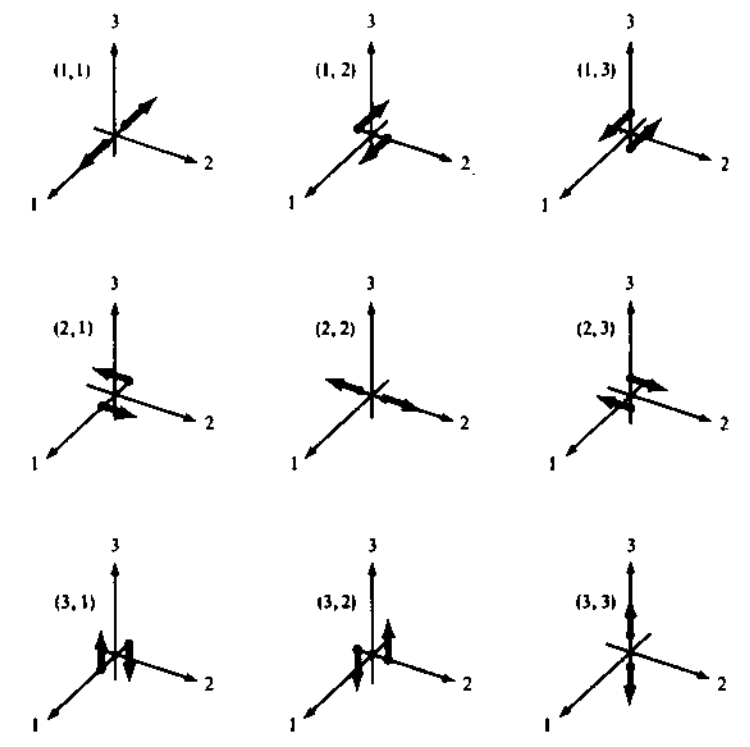
\includegraphics[scale=0.4]{figures/MomentTensor}
\centering
\caption{Unit force couples, $\boldsymbol{\hat{F}}^{(i,j)}$, that can
  be used to represent any type of dislocation on a fault (taken from
  \citet{AR2002})}

\end{figure}

\section*{Spectral Discretization}
We will assume, for computational tractability but without loss of
generality, that the domain is a two dimensional cross-section of the
Earth and displacements are only in the plane of that cross-section.
After expanding the summation notation, eq. (\ref{DiffEq}) can then be
written as
\begin{equation}
\begin{vmatrix}
  \partial^2 u_1/\partial t^2\\ \\
  \partial^2 u_2/\partial t^2
\end{vmatrix} =
\begin{vmatrix}
 \partial_1\left((\lambda + 2\mu)\partial_1 u_1\right) +  
 \partial_2\left(\mu\partial_2 u_1\right) + 
 \partial_1\left(\lambda\partial_2 u_2\right) +  
 \partial_2\left(\mu\partial_1 u_2\right)\\ \\
 \partial_1\left(\mu\partial_2 u_1\right) +  
 \partial_2\left(\lambda\partial_1 u_1\right) + 
 \partial_2\left((\lambda + 2\mu)\partial_2 u_2\right) +  
 \partial_1\left(\mu\partial_1 u_2\right) 
\end{vmatrix} + 
\begin{vmatrix}
  f_1\\ \\
  f_2
\end{vmatrix},
\end{equation}
where we use $\partial_i$ to denote a derivative with respect to
$x_i$.  Likewise, the boundary conditions can be written as
\begin{equation}
\begin{vmatrix}
  0\\ \\
  0
\end{vmatrix} =
\begin{vmatrix}
 \hat{n}_1(\lambda + 2\mu)\partial_1 u_1 +  
 \hat{n}_2\mu\partial_2 u_1 + 
 \hat{n}_1\lambda\partial_2 u_2 +  
 \hat{n}_2\mu\partial_1 u_2\\ \\
 \hat{n}_1\mu\partial_2 u_1 +  
 \hat{n}_2\lambda\partial_1 u_1 + 
 \hat{n}_2(\lambda + 2\mu)\partial_2 u_2 +  
 \hat{n}_1\mu\partial_1 u_2
\end{vmatrix} 
\end{equation}

We chose to solve eq. (\ref{DiffEq}) in the spatial dimension using
multiquadratic radial basis functions, which are defined as
\begin{equation}\label{RBF}
  \phi(\boldsymbol{x}) = \sqrt{1 + (\epsilon|\boldsymbol{x} - \boldsymbol{x}_o|)^2}. 
\end{equation}
In the above equation $\epsilon$ is the shape parameter and
$\boldsymbol{x}_o$ is the center of the RBF.  We chose to use
multiquadratic radial basis functions because interpolating a function
using $\phi(\boldsymbol{x})$ has the desirable trait of being
equivalent to piece-wise linear interpolation for $\epsilon \to
\infty$ and polynomial interpolation for $\epsilon \to 0$ at least for
one-dimensional problems \citep{D2002}.  This suggests that a wide
range of values for $\epsilon$ should produce reasonably accurate
results because either end-member is a perfectly valid means of
interpolation.  This is in contrast to using RBFs that decay to zero
as $|\boldsymbol{x - x_o}| \to \infty$, where the interpolant for $\epsilon
\to \infty$ is essentially useless.  We follow the common practice of
making $\epsilon$ for each RBF proportional to the distance to the
nearest RBF center.  We did not rigorously search for an optimal
proportionality constant; however, we note that we tend to get
unstable or obviously inaccurate solutions for proprtionality
constants greater than $2$ and less than $0.1$.  For the solution
presented in this paper, we used a proportionality constant of 1, that
is, we set $\epsilon$ equal to the distance to the nearest neighbor.

We approximate the solution for displacements as 
\begin{equation}
  u_1 \approx \sum_{j=1}^{N}\alpha_{j}(t)\phi_j(\boldsymbol{x})
\end{equation}
and
\begin{equation}
  u_2 \approx \sum_{j=1}^{N}\beta_{j}(t)\phi_j(\boldsymbol{x}),
\end{equation}
which can also be written as 
\begin{equation}
\begin{vmatrix}
  u_1 \\
  u_2 
\end{vmatrix} \approx 
\boldsymbol{G}
\begin{vmatrix}
  \boldsymbol{\alpha}\\
  \boldsymbol{\beta}
\end{vmatrix}
\end{equation}
where $\boldsymbol{G}$ is given by
\begin{equation}
\boldsymbol{G} = 
\begin{vmatrix}
\boldsymbol{\phi}&\boldsymbol{0}\\
\boldsymbol{0}&\boldsymbol{\phi}
\end{vmatrix}
\end{equation}
and we are no longer explicitly writing the time and space dependence.
We can then express acceleration in terms of the spectral
coefficients, $\boldsymbol{\alpha}$ and $\boldsymbol{\beta}$, as
\begin{equation}\label{Acceleration}
\begin{vmatrix}
  \partial^2 u_1/\partial t^2\\
  \partial^2 u_2/\partial t^2
\end{vmatrix} =
\boldsymbol{H}
\begin{vmatrix}
  \boldsymbol{\alpha}\\
  \boldsymbol{\beta}
\end{vmatrix} + 
\begin{vmatrix}
  f_1\\
  f_2
\end{vmatrix},
\end{equation}
where
\begin{equation}
\boldsymbol{H} = 
\begin{vmatrix}
 \partial_1\left((\lambda + 2\mu)\partial_1 \boldsymbol{\phi}\right) +  
 \partial_2\left(\mu\partial_2 \boldsymbol{\phi}\right)&
 \partial_1\left(\lambda\partial_2 \boldsymbol{\phi}\right) +  
 \partial_2\left(\mu\partial_1 \boldsymbol{\phi}\right)\\
 \partial_1\left(\mu\partial_2 \boldsymbol{\phi}\right) +  
 \partial_2\left(\lambda\partial_1 \boldsymbol{\phi}\right)&
 \partial_2\left((\lambda + 2\mu)\partial_2 \boldsymbol{\phi}\right) +  
 \partial_1\left(\mu\partial_1 \boldsymbol{\phi}\right) 
\end{vmatrix}.
\end{equation}
The boundary conditions can also be expressed in terms of the spectral
coefficients as
\begin{equation}
\begin{vmatrix}
  0\\
  0
\end{vmatrix} =
\boldsymbol{B}
\begin{vmatrix}
  \boldsymbol{\alpha}\\
  \boldsymbol{\beta}
\end{vmatrix},
\end{equation}
where
\begin{equation}
\boldsymbol{B} = 
\begin{vmatrix}
 \hat{n}_1(\lambda + 2\mu)\partial_1 \boldsymbol{\phi} +  
 \hat{n}_2\mu\partial_2 \boldsymbol{\phi} &
 \hat{n}_1\lambda\partial_2 \boldsymbol{\phi} +  
 \hat{n}_2\mu\partial_1 \boldsymbol{\phi}\\
 \hat{n}_1\mu\partial_2 \boldsymbol{\phi} +  
 \hat{n}_2\lambda\partial_1 \boldsymbol{\phi} &
 \hat{n}_2(\lambda + 2\mu)\partial_2 \boldsymbol{\phi} +  
 \hat{n}_1\mu\partial_1 \boldsymbol{\phi}
\end{vmatrix}.
\end{equation}
At this point, all the information in $\boldsymbol{G}$,
$\boldsymbol{H}$, $\boldsymbol{B}$, and $\boldsymbol{f}$ are given by
the problem description or are user defined variables.  Finding the
spectral coefficients for $\boldsymbol{u}$ is then straightforward.
We perform the time integration with a leapfrog method and our
procedure for solving eq. (\ref{DiffEq}) is as follows:
\begin{enumerate}
\item Form the matrix $\boldsymbol{J}$, which consists of
  $\boldsymbol{B}$ evaluated at the boundary collocation points and 
  $\boldsymbol{G}$ evaluated at the interior collocation points.
\item Form the vector $\boldsymbol{r}^0$, which consists of zeros for
  the boundary collocation points and $\boldsymbol{u}^{0}$ at the interior collocation points 
\item Solve $\boldsymbol{r}^0=\boldsymbol{J}[\boldsymbol{\alpha}^0\ \boldsymbol{\beta}^0]^T$ for
  $\boldsymbol{\alpha}^0$ and $\boldsymbol{\beta}^0$
\item evaluate the initial acceleration, $\boldsymbol{a}^0$, using eq. (\ref{Acceleration}) 
\item begin time stepping 
\begin{enumerate}
\item evaluate $\boldsymbol{u}^{t}=\boldsymbol{u}^{t-1} + 
                                  \boldsymbol{v}^{t-1}\Delta t + 
                                  \boldsymbol{a}^{t-1}\Delta t^2$
\item Form $\boldsymbol{r}^t$
\item Solve $\boldsymbol{r}^t=\boldsymbol{J}[\boldsymbol{\alpha}^t\ \boldsymbol{\beta}^t]^T$ for
  $\boldsymbol{\alpha}^t$ and $\boldsymbol{\beta}^t$
\item evaluate $\boldsymbol{a}^t$ from eq. (\ref{Acceleration})
\item evaluate $\boldsymbol{v}^t = \boldsymbol{v}^{t-1} +
  1/2(\boldsymbol{a}^{t-1} + \boldsymbol{a}^t)\Delta t$
\end{enumerate} 
\end{enumerate} 

There are, however, a few additional details that need to be
addressed.  First, we must deal with the material properties, $\mu$,
$\lambda$, and $\rho$.  We use the material properties from the
Preliminary Reference Earth Model (PREM) \citep{D1981}.  PREM was
inferred using observed P and S wave travel times in addition to other
geophysical data.  We then have a means of validating our numerical
solution because the travel times predicted by our numerical
simulation should be consistent with observable travel times.  The
material properties for PREM are given at discrete depths, and so we
perform an interpolation using multiquadratic RBFs to obtain PREM as a
continuous and analytically differentiable function.  Our interpolants
for PREM are shown in figure 2, 3, and 4.

\begin{figure}[h!]
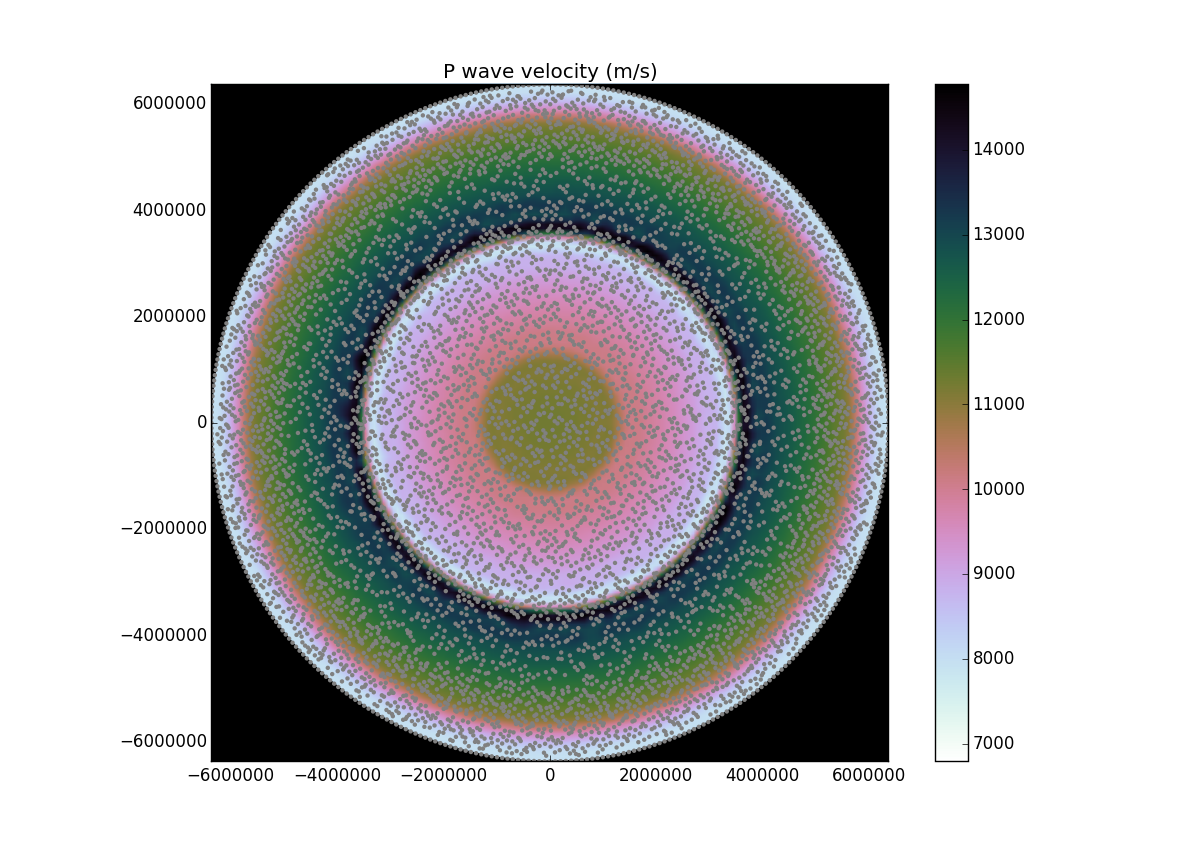
\includegraphics[scale=0.5]{figures/Pvel}
\centering
\caption{P wave velocities ($\sqrt{(\lambda + 2\mu)/\rho}$) from PREM.
  Gray dots indicate collocation points used in solving
  eq. (\ref{DiffEq})}

\end{figure}
\begin{figure}[h!]
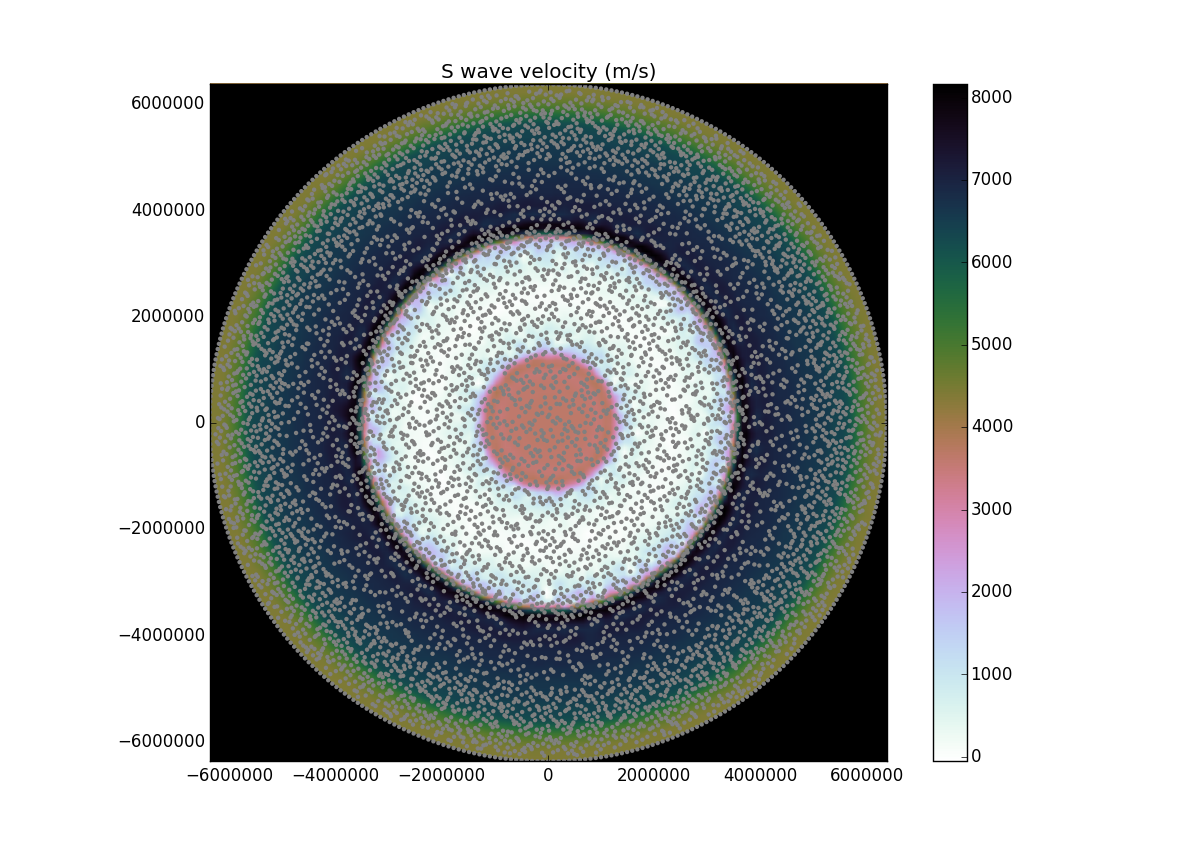
\includegraphics[scale=0.5]{figures/Svel}
\centering
\caption{S wave velocities ($\sqrt{\mu/\rho}$) from PREM}

\end{figure}
\begin{figure}[h!]
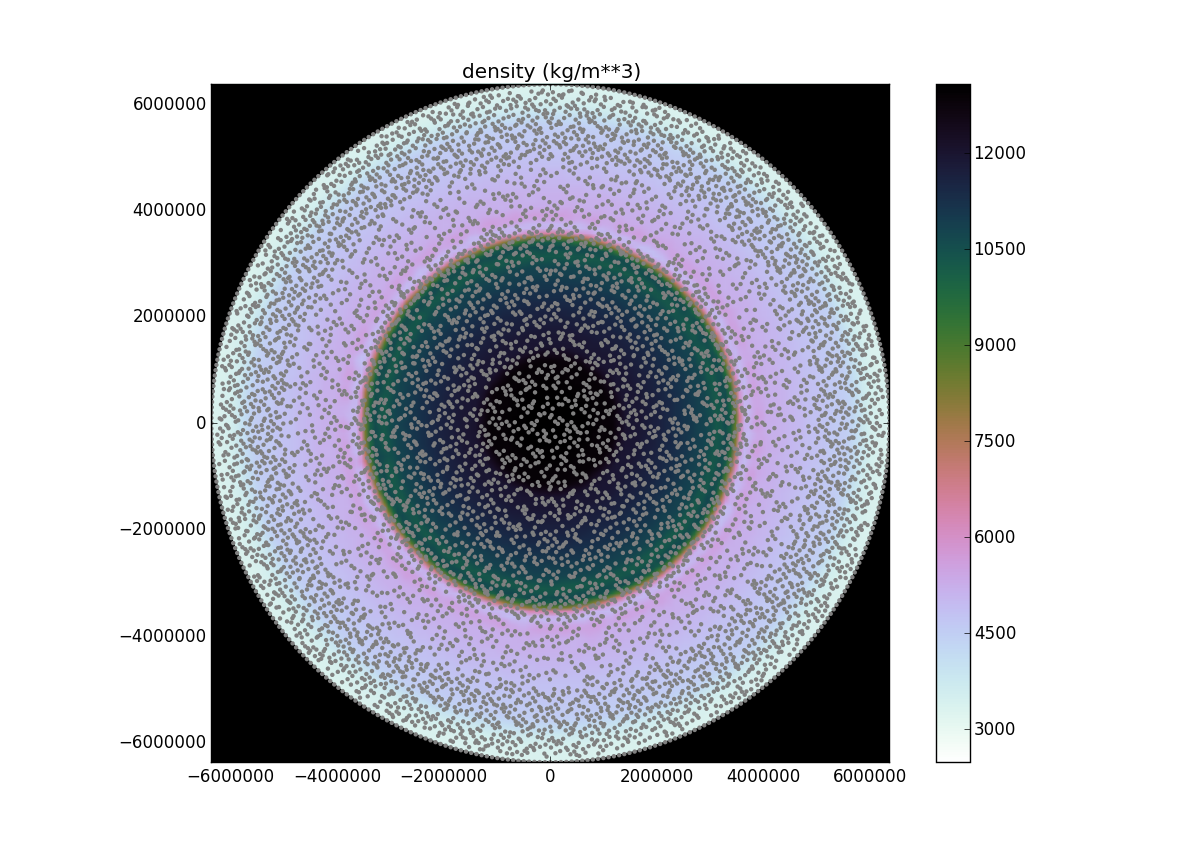
\includegraphics[scale=0.5]{figures/density}
\centering
\caption{Densities from PREM}

\end{figure}

We also must address how the collocation points are chosen.  PREM has
a major material disontinuity at the core-mantle boundary and we would
ideally prefer to have a higher density of nodes at that interface.
Additionally, the lower mantle has higher P and S wave velocities
relative to the upper mantle, crust, and core.  We would then prefer a
lower density of collocation points in the lower mantle in order to
keep our solution stable during time stepping.  Although we seek
regional scale variations in node density, we still want our
collocation points to have low discrepency in any given region of the
earth.  We have developed a simple method to produce a distribution of
collocation points that satisfy our specifications.  Let
$\psi:\boldsymbol{x}\to [0,1]$ be a normalized function describing the
desired density of collocation points at position $\boldsymbol{x}$.
Let $H^1_k$ be the $k^{th}$ element in a one-dimensional Halton
sequence.  Let $H^2_k$ be the $k^{th}$ element of a two-dimensional
Halton sequence which has been scaled so that $H^2_k$ can lie anywhere
in the problem domain, $D$. The set of $N$ collocation points,
$\boldsymbol{C}$, with the desired density can then be found with algorithm 1.

In our experience, we found that it is necessary to have a small
buffer between the boundary collocation points and interior
collocation points.  This is essential for a stable solution.  We take
the width of the buffer to be the smallest distance between boundary
nodes.  The reader may be able to notice this slight buffer in either
Figures 2, 3 or 4.

\begin{algorithm}[h!]
\caption{Collocation points}
\begin{algorithmic}
\STATE $\boldsymbol{C} = \emptyset$
\STATE $k = 0$
\WHILE{(length of $\boldsymbol{C}) < N$}
  \IF{($\phi(H^2_k) > H^1_k) \& (H^2_k \in D)$}
    \STATE append $H^2_k$ to $\boldsymbol{C}$
  \ENDIF
  \STATE $k = k + 1$  
\ENDWHILE
\end{algorithmic}
\end{algorithm}
\section*{Results}
Our numerical solution to eq. (\ref{DiffEq}) is shown in figures 2-10.
The most prominent feature in our solution are the Raleigh waves which
travel along the surface and have decaying amplitude with depth.  The
fastest traveling waves are the P waves which have only a faint
signature.  We can also be assured that the material properties are
properly implemented because S waves, which have displacements
parallel to the wave front, do not enter the core because it has a
shear wave velocity of zero.

It is also worth noting that the solution has symmetry about the
vertical axis.  This symmetry is no suprise and we have attemted to
solve eq. (\ref{DiffEq}) on only half the domain.  However, we have
found that solutions using RBFs are incredibly sensitive to corners in
the domain and our solution quickly went unstable after a few time
steps.

We note that the magnitude of displacements in our solution is far
larger than what we would reasonably expect.  We believe this to be a
bug in our program that is related to unit conversions and the actual
solution should be different by only a constant factor.

We can also verify the accuracy of our solution by ensuring that it is 
symmetric

\begin{figure}
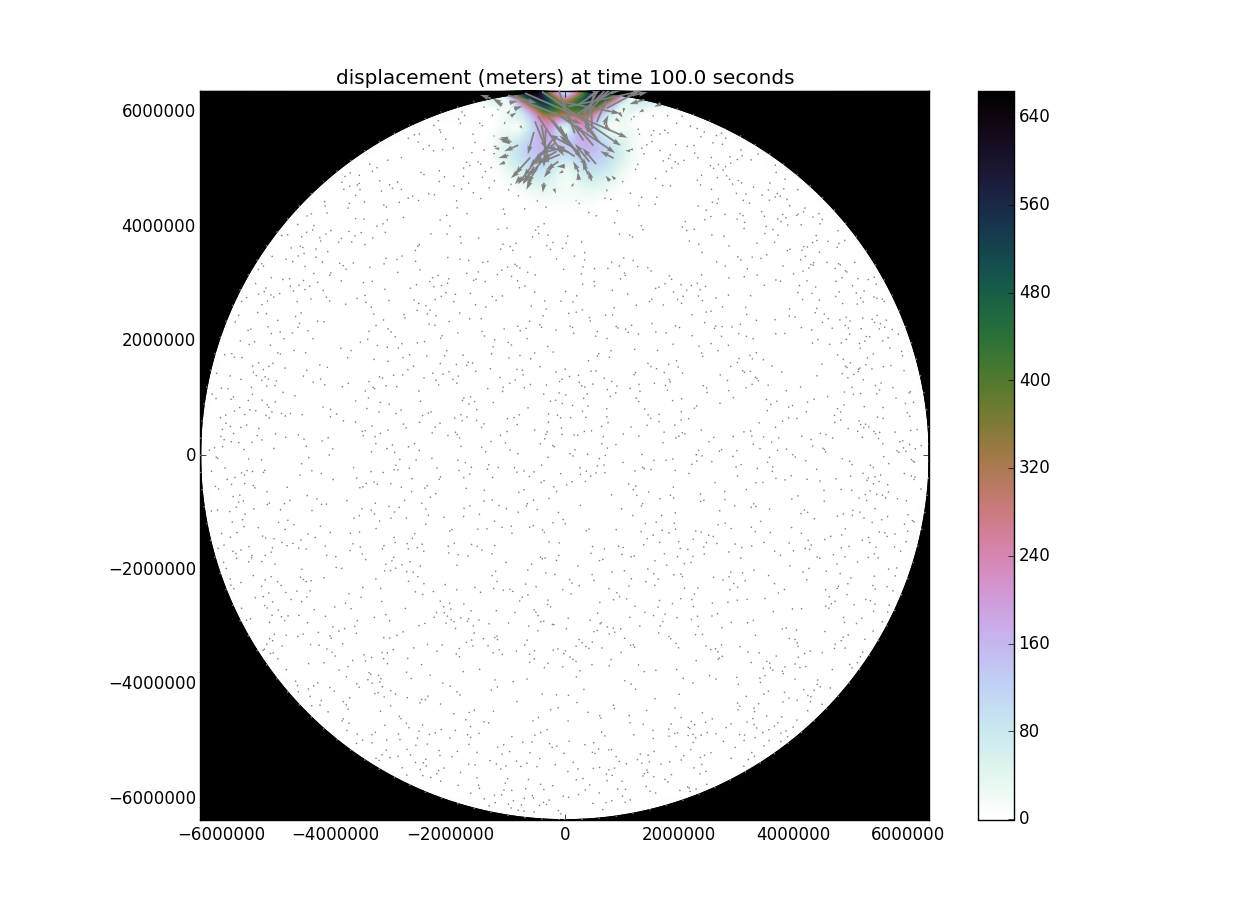
\includegraphics[scale=0.45]{figures/100s}
\centering
\caption{Solution for displacements at 100 seconds after an earthquake. Color
  indicates the magnitude of displacement and vectors indicate
  direction}
\end{figure}
\begin{figure}
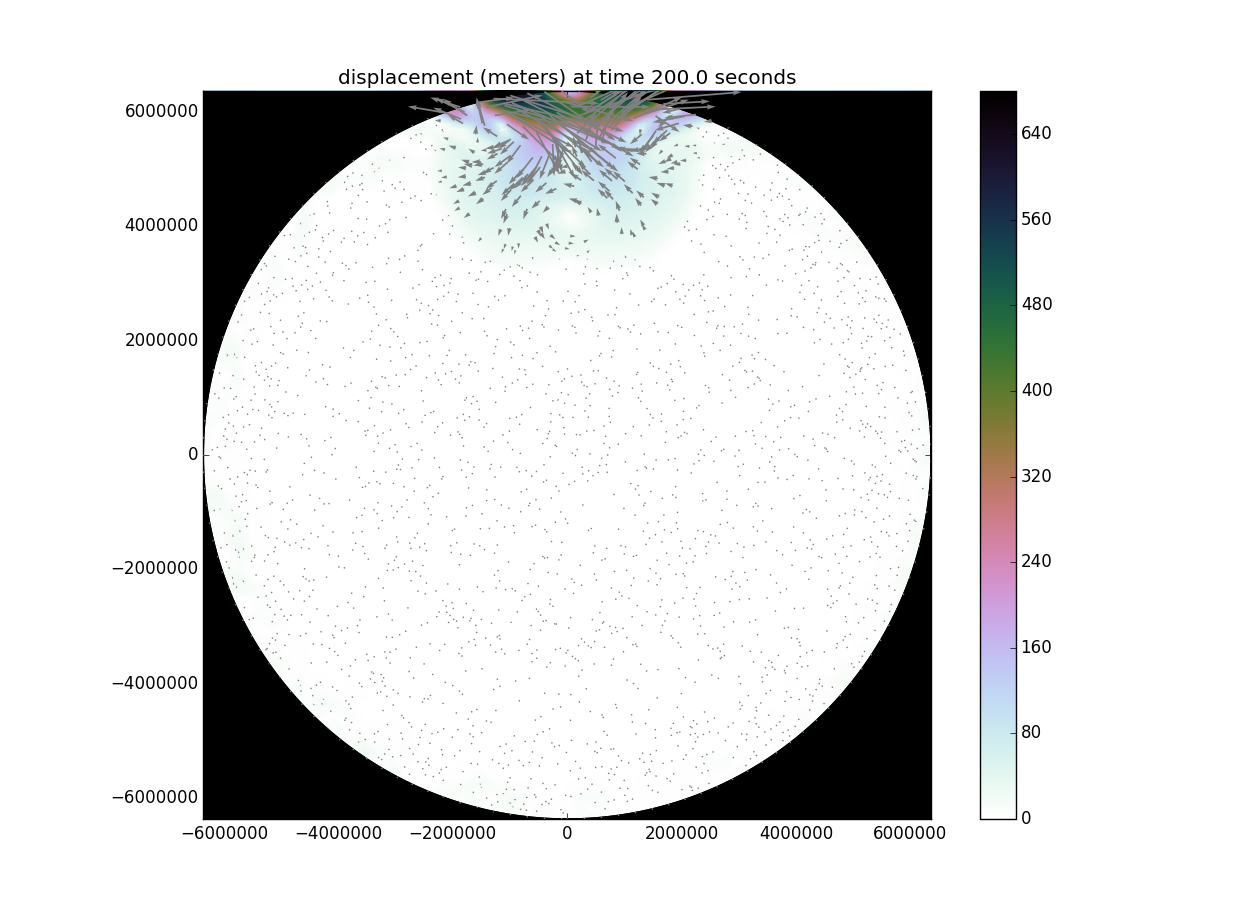
\includegraphics[scale=0.45]{figures/200s}
\centering
\caption{Solution for displacements at 200 seconds after an earthquake}

\end{figure}
\begin{figure}
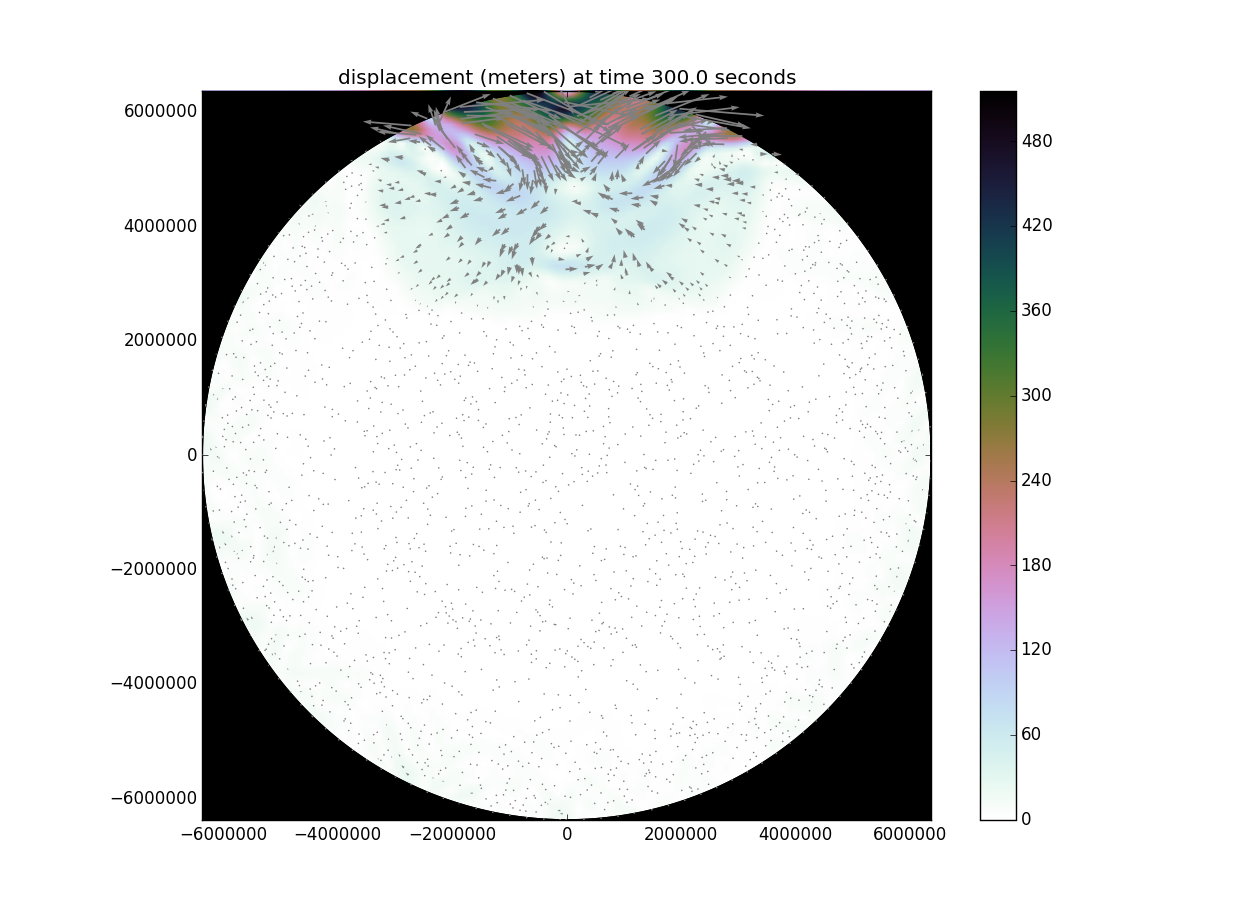
\includegraphics[scale=0.45]{figures/300s}
\centering
\caption{Solution for displacements at 300 seconds after an earthquake}

\end{figure}
\begin{figure}
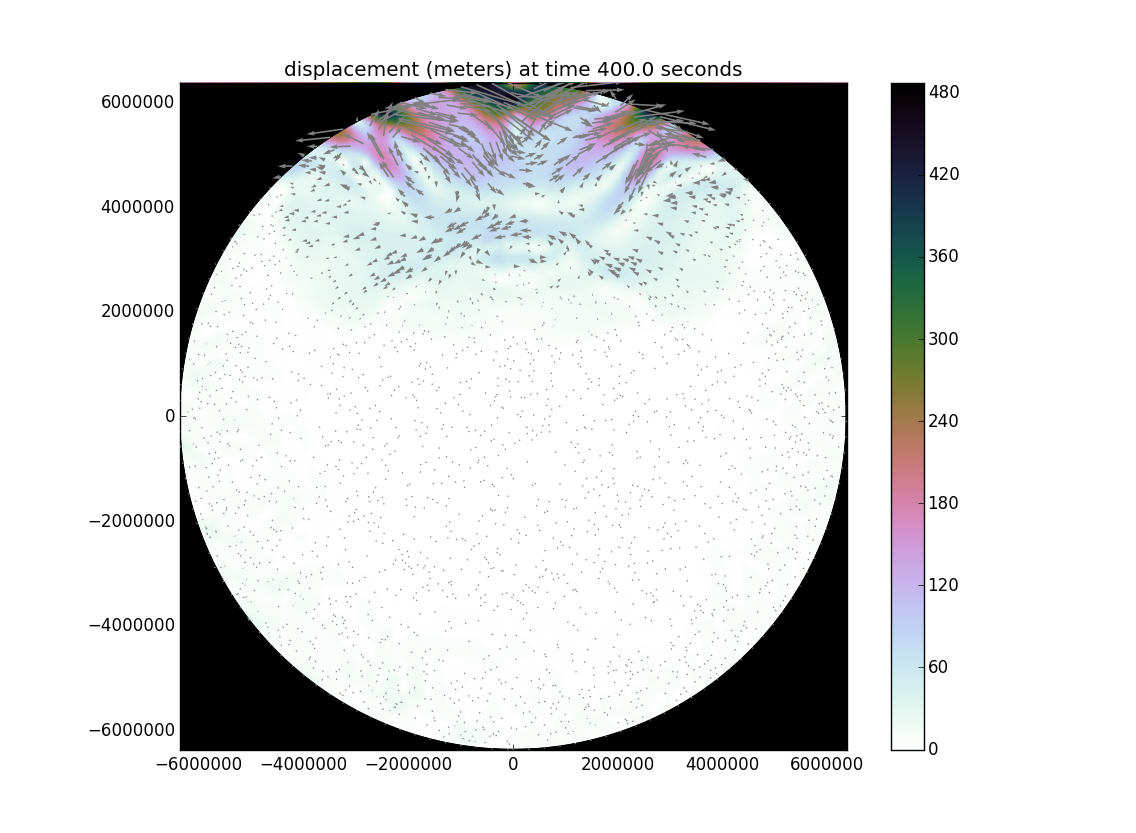
\includegraphics[scale=0.45]{figures/400s}
\centering
\caption{Solution for displacements at 400 seconds after an earthquake}

\end{figure}
\begin{figure}
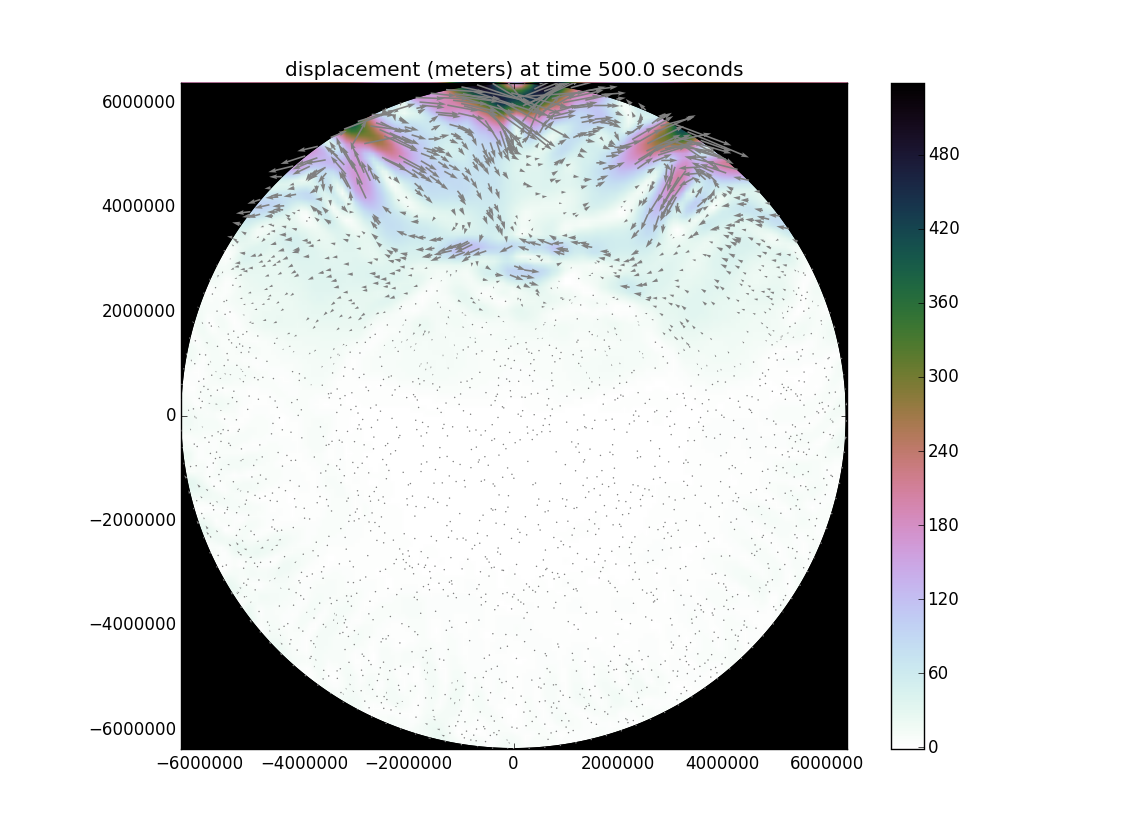
\includegraphics[scale=0.45]{figures/500s}
\centering
\caption{Solution for displacements at 500 seconds after an earthquake}
\end{figure}

\section*{Additional notes}
  All the software that I have written to produce the results shown in
  this paper are included below.  The software (with eventual bug
  fixes) can also be found at https://github.com/treverhines/SeisRBF
  My software uses packages which can be found in the Anaconda Python
  distribution from Continuum Analytics.  

%\pythonscript{Lab03_snippet}{Lab03.py} 

\begin{thebibliography}{}
  \bibitem[Aki \& Richards(2002)]{AR2002} Aki, K. \& Richards, P.,
    2002. Quantitative Seismology, second edition, \textit{University
      Science Books}


  \bibitem[Driscoll \& Fornberg(2002)]{D2002} Driscoll, T. \& Fornberg, B.,
    2002. Interpolation in the limit of increasingly fiat radial basis
    functions, \textit{Computers and Mathematics with Applications},
    43, 413-422.

  \bibitem[Dziewonski \& Anderson(1981)]{D1981} Dziewonski, A. M. \&
    Anderson, D.L., 1981. Preliminary reference Earth
    model. \textit{Phys Earth Planet Inter}, 25,
    297-356. doi:10.1016/0031-9201(81)90046-7.

  \bibitem[Fichtner(2011)]{F2011} Fichtner, A., 2011. Full Seismic
    Waveform Modelling and Inversion, \textit{Springer}
\end{thebibliography}
\end{document}

